% CMPE 249 project talk (10 min). Build: tectonic slides/talk.tex  (or latexmk -xelatex)
% Figures: python hpc/talk_figures.py runs/analysis slides/figures
\documentclass[aspectratio=169,11pt]{beamer}
\usetheme{default}
\usepackage{tikz,booktabs,xcolor}
\usetikzlibrary{arrows.meta,positioning,fit,backgrounds}
\graphicspath{{figures/}}

\definecolor{ink}{HTML}{1D232B}\definecolor{muted}{HTML}{5A6270}\definecolor{paper}{HTML}{FBFAF7}
\definecolor{demo}{HTML}{2A78D6}\definecolor{rand}{HTML}{EB6834}\definecolor{icm}{HTML}{1BAF7A}
\definecolor{accent}{HTML}{C2410C}\definecolor{soft}{HTML}{EEF2F7}
\setbeamercolor{background canvas}{bg=paper}
\setbeamercolor{normal text}{fg=ink}\setbeamercolor{frametitle}{fg=ink}\setbeamercolor{title}{fg=ink}
\setbeamercolor{itemize item}{fg=accent}\setbeamercolor{alerted text}{fg=accent}
\setbeamerfont{frametitle}{size=\Large,series=\bfseries}
\setbeamertemplate{navigation symbols}{}
\setbeamertemplate{itemize item}{\small$\blacktriangleright$}
\setbeamertemplate{footline}{\hfill\textcolor{muted}{\scriptsize\insertframenumber\hspace{1.2em}}\vspace{0.6em}}
\newcommand{\pending}[1]{\textcolor{accent}{\textbf{[#1]}}}
\newcommand{\src}[1]{\par\vfill\textcolor{muted}{\scriptsize #1}}

\title{Does the source of exploration data matter\\for fine-tuning a small VLA?}
\author{Aaron Chandler}
\institute{CMPE 249 Intelligent Autonomous Systems \textbullet{} San Jos\'e State University\\[2pt]\texttt{github.com/AaronChandler976/curious-vla}}
\date{December 2026}

\begin{document}

\begin{frame}[plain]
\titlepage
\end{frame}

% ---------------------------------------------------------------- 1. problem
\begin{frame}{Demonstrations are the bottleneck; robot play is free}
\begin{columns}[T]
\column{0.55\textwidth}
\begin{itemize}\setlength\itemsep{0.8em}
\item VLA policies learn manipulation from \textbf{teleoperated demos}: slow, expensive, task-specific.
\item A robot can \textbf{explore on its own} for free, but that data has no task label and no reward.
\item Setting: a small VLA (SmolVLA, 450M params, fits a single GPU) fine-tuned with only 10--40 demos per task.
\end{itemize}
\column{0.42\textwidth}
\begin{block}{Question}
At the same amount of collected data, does \textbf{curiosity-driven} exploration give a VLA more than \textbf{random} exploration, or than no exploration at all?
\end{block}
\end{columns}
\end{frame}

% ---------------------------------------------------------------- 2. landscape
\begin{frame}{What already exists}
\small
\begin{tabular}{@{}p{0.2\textwidth}p{0.42\textwidth}p{0.32\textwidth}@{}}
\toprule
\textbf{Work} & \textbf{Shows} & \textbf{Gap left} \\ \midrule
World-Env (2025) & Exploration from a perturbed trained policy helps OpenVLA-OFT on LIBERO, via RL in a world model & Source is a competent policy; channel is RL \\
TAP (ICML 2026) & 30 h of random play + inverse-dynamics pretraining: +10 pts on SIMPLER & One source only; not plain BC \\
ExORL (2022) & For offline RL, \emph{which} explorer collected the data matters a lot & Needs reward labels \\
Negative transfer (2026) & Mismatched data under action-only loss can hurt a VLA & No exploration study \\ \bottomrule
\end{tabular}
\vspace{0.8em}

\textbf{Gap:} no comparison of exploration \emph{sources} as fine-tuning data for a VLA under matched budgets.\\
\textcolor{muted}{Scope set with the professor: 3 conditions, 2 tasks; VLM-guided curiosity is a stretch goal.}
\end{frame}

% ---------------------------------------------------------------- 3. method
\begin{frame}{Pipeline: one data path for every condition}
\centering
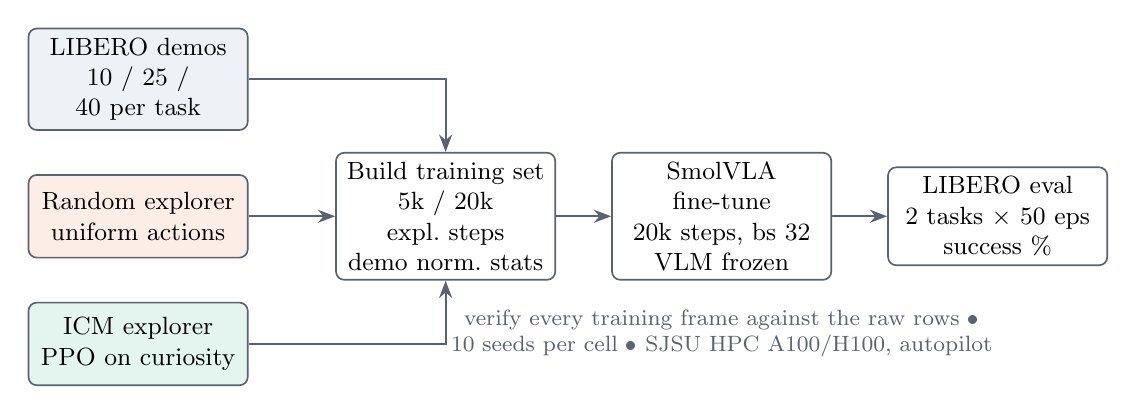
\begin{tikzpicture}[font=\small, node distance=0.55cm and 0.7cm,
  box/.style={draw=muted, rounded corners=3pt, fill=white, align=center, minimum height=1.05cm, text width=2.55cm, line width=0.6pt},
  arr/.style={-{Stealth[length=2.2mm]}, line width=0.8pt, draw=muted}]
\node[box, fill=soft] (demo) {LIBERO demos\\10 / 25 / 40 per task};
\node[box, below=of demo, fill=rand!12] (rnd) {Random explorer\\uniform actions};
\node[box, below=of rnd, fill=icm!12] (icm) {ICM explorer\\PPO on curiosity};
\node[box, right=1.1cm of rnd] (build) {Build training set\\5k / 20k expl.\ steps\\demo norm.\ stats};
\node[box, right=of build] (train) {SmolVLA fine-tune\\20k steps, bs 32\\VLM frozen};
\node[box, right=of train] (eval) {LIBERO eval\\2 tasks $\times$ 50 eps\\success \%};
\draw[arr] (demo) -| (build); \draw[arr] (rnd) -- (build); \draw[arr] (icm) -| (build);
\draw[arr] (build) -- (train); \draw[arr] (train) -- (eval);
\node[below=0.25cm of train, text width=7.6cm, align=center, text=muted, font=\footnotesize] (v)
 {verify every training frame against the raw rows \textbullet{} 10 seeds per cell \textbullet{} SJSU HPC A100/H100, autopilot};
\end{tikzpicture}
\vspace{0.4em}
\begin{itemize}\small
\item \textbf{Matched budgets:} same env steps of exploration, same training steps, base model, normalization and eval seeds.
\item Exploration frames get the instruction ``explore the scene''; demos keep theirs. Mix = 50\% exploration frames.
\end{itemize}
\end{frame}

% ---------------------------------------------------------------- 4. engineering
\begin{frame}{Getting a trustworthy pipeline}
\begin{columns}[T]
\column{0.5\textwidth}
\textbf{Bugs that would have silently ruined results}
\begin{itemize}\small\setlength\itemsep{0.4em}
\item Fine-tuning from \texttt{smolvla\_base} kept its 6-D state and wrong cameras: normal loss, 0\% success. Fixed by copying LIBERO's feature spec; checked in a CPU dry run.
\item The cached LIBERO dataset's episode index pointed at the wrong rows; every training set is now rebuilt from raw rows and verified.
\item Bad GPU / rendering nodes: jobs self-check and resubmit elsewhere.
\end{itemize}
\column{0.46\textwidth}
\textbf{Scale}
\begin{itemize}\small\setlength\itemsep{0.4em}
\item 464 fine-tunes planned (224 done, 240 running)
\item 1.0 h per 20k-step fine-tune on H100 (1.6 h on A100), 7.7 GB peak
\item Official \texttt{smolvla\_libero} scores 64\% on these tasks through our eval (others report $\approx$66\% on LIBERO-Object for the public checkpoint)
\end{itemize}
\end{columns}
\end{frame}

% ---------------------------------------------------------------- 5. main result
\begin{frame}{Result 1: no exploration mix beats demos only}
\centering
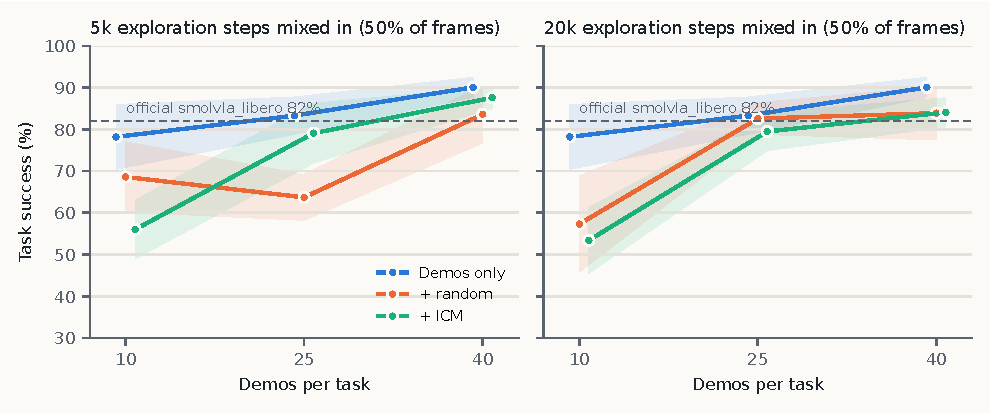
\includegraphics[width=0.96\textwidth]{c1_main.pdf}
\small Mean of 10 seeds, 95\% CI. Pooled change vs demos only: random $-14$ / $-6$, ICM $-2$ / $-19$ pts (5k / 20k).
\end{frame}

% ---------------------------------------------------------------- 6. ICM vs random
\begin{frame}{Result 2: ICM vs random flips sign; the data draw matters as much}
\centering
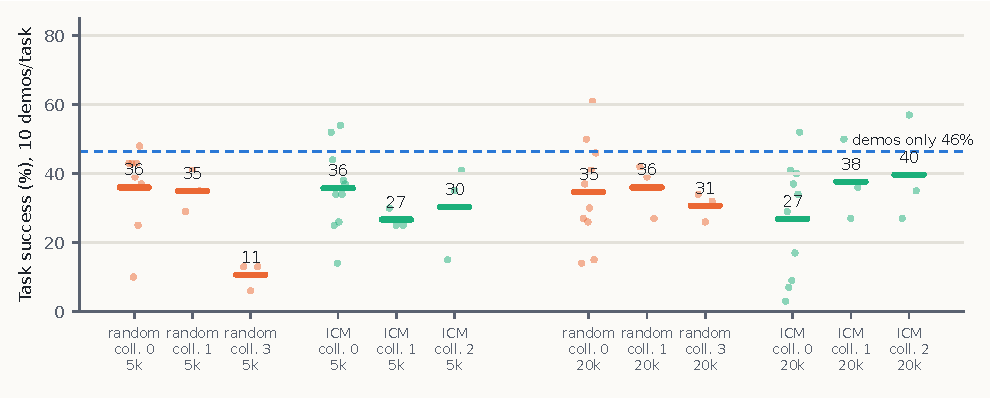
\includegraphics[width=0.93\textwidth]{c2_replicates.pdf}
\small ICM $-$ random: \textbf{+12} pts at 5k, \textbf{$-13$} pts at 20k (paired, 30 pairs each). Re-collecting the \emph{same} method's data moves success by up to 25 pts. Every collection is below demos only.
\end{frame}

% ---------------------------------------------------------------- 7. diagnosis: what is in the data
\begin{frame}{Why: the exploration data has nothing a BC loss can learn}
\begin{columns}[T]
\column{0.6\textwidth}\footnotesize
\begin{tabular}{@{}lrrr@{}}\toprule
 & Demos & Random & ICM \\ \midrule
Action predictable from state ($R^2$) & 0.42 & $\le$0.01 & $\le$0.01 \\
Frames within 3 cm of demo paths & 100\% & 13--18\% & 11--18\% \\
Episodes that move an object & 100\% & 44--58\% & 36--84\% \\
2 cm voxels visited (20k steps) & -- & 10.2k & 12.8k \\
Mean $|$action$|$ & 0.16 & 0.50 & 0.63 \\
PPO updates / policy std & -- & -- & 7 / 1.00 \\ \bottomrule
\end{tabular}
\column{0.37\textwidth}\footnotesize
\begin{itemize}\setlength\itemsep{0.5em}
\item SmolVLA trains only the action expert; the VLM is frozen. Exploration can only teach \emph{actions}.
\item Its actions are unpredictable from what the robot sees, so BC learns noise.
\item The ICM policy \alert{barely trained}: it differed from random mainly in action scale, not curiosity.
\end{itemize}
\end{columns}
\end{frame}

% ---------------------------------------------------------------- 8. falsification
\begin{frame}{Falsification tests (running on HPC now)}
\small
\begin{tabular}{@{}p{0.27\textwidth}p{0.36\textwidth}p{0.3\textwidth}@{}}\toprule
\textbf{Test} & \textbf{If \dots} & \textbf{Result} \\ \midrule
Dilution control: demos only, 10k steps (= demo exposure of a 50\% mix) & mix $\approx$ it: exploration is inert; mix $<$ it: exploration actively hurts & \pending{Nov 30} \\
Exploration first, then demos (TAP order, BC loss) & beats demos-10k: exploration has value through pretraining & \pending{Nov 30} \\
ICM with 150k-step warm-up (230 PPO updates) & beats random: curiosity matters once it is trained & \pending{Nov 30} \\
3 collections per method & ICM$-$random holds across collections & \pending{Nov 30} \\
Mixing share 10 / 25 / 50\% & harm grows with the share & at 10\% back to demos-only level \\ \bottomrule
\end{tabular}
\vspace{0.6em}

Decision rule: call a difference zero only if its paired 95\% CI lies within $\pm$5 pts.
\end{frame}

% ---------------------------------------------------------------- 9. ratio
\begin{frame}{Ablation: how much exploration to mix in}
\centering
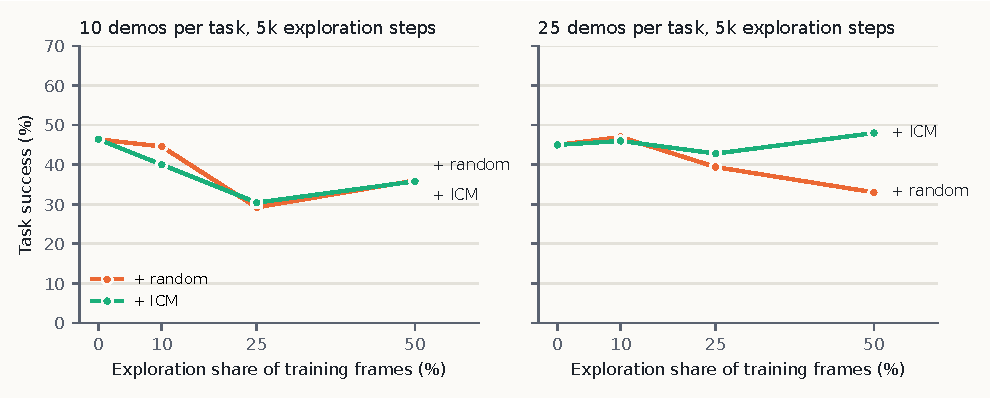
\includegraphics[width=0.93\textwidth]{c3_ratio.pdf}
\small 5 seeds at 10\% and 25\%, 10 at 50\%. No share beats demos only; small shares are harmless.
\end{frame}

% ---------------------------------------------------------------- 10. cost
\begin{frame}{Latency and resources}
\small
\begin{columns}[T]
\column{0.48\textwidth}
\textbf{Training} (per fine-tune, batch 32)\\[0.3em]
\begin{tabular}{@{}lrr@{}}\toprule
GPU & s/step & 20k steps \\ \midrule
H100 PCIe & 0.17 & 0.96 h \\
H100 NVL & 0.18 & 1.02 h \\
A100 40GB & 0.28 & 1.57 h \\ \bottomrule
\end{tabular}\\[0.3em]
Peak memory 7.7 GB; 100M of 450M params trainable.
\column{0.48\textwidth}
\textbf{Inference} (one 50-step action chunk)\\[0.3em]
\pending{A100/H100 latency, ms per chunk and per step}\\[0.5em]
\textbf{Data collection}\\[0.3em]
20k exploration steps in $\approx$32 min (10 steps/s, rendering bound); trained ICM adds a 150k-step warm-up.
\end{columns}
\end{frame}

% ---------------------------------------------------------------- 11. insights
\begin{frame}{What I learned}
\begin{itemize}\setlength\itemsep{0.7em}
\item \textbf{Negative result:} mixing task-free exploration into SmolVLA fine-tuning the default way costs up to 19 points. Don't do it.
\item The \textbf{data source} question can't be answered with one collection per method: re-collecting moves results as much as switching methods.
\item The \textbf{training channel} matters more than the explorer: with a frozen VLM and a BC loss, unlabeled actions are noise. TAP's inverse-dynamics loss is the channel that works.
\item \textbf{Next:} inverse-dynamics pretraining on the same data, a trained curiosity explorer, unfreezing the VLM.
\end{itemize}
\end{frame}

\begin{frame}[plain]
\centering\Large Thank you\\[1em]
\normalsize\texttt{github.com/AaronChandler976/curious-vla}
\end{frame}

\end{document}
